\def\year{2018}\relax
%File: formatting-instruction.tex
\documentclass[letterpaper]{article} %DO NOT CHANGE THIS
\usepackage{aaai18}  %Required
\usepackage{times}  %Required
\usepackage{helvet}  %Required
\usepackage{courier}  %Required
\usepackage{url}  %Required
\usepackage{graphicx}  %Required
\frenchspacing  %Required
\usepackage[utf8]{inputenc} % allow utf-8 input
\usepackage[T1]{fontenc}    % use 8-bit T1 fonts
\usepackage{hyperref}       % hyperlinks
\usepackage{url}            % simple URL typesetting
\usepackage{booktabs}       % professional-quality tables
\usepackage{amsfonts}       % blackboard math symbols
\usepackage{nicefrac}       % compact symbols for 1/2, etc.
\usepackage{microtype}      % microtypography

\usepackage{amsmath}
\usepackage{subcaption}
\usepackage{mathrsfs} 
\usepackage{cancel}
\usepackage{amsfonts}
\usepackage[titletoc,title]{appendix}
\usepackage{floatrow}
\usepackage[draft]{todonotes}   % notes showed
\usepackage[]{algorithm2e}

\setlength{\pdfpagewidth}{8.5in}  %Required
\setlength{\pdfpageheight}{11in}  %Required
%PDF Info Is Required:
  \pdfinfo{
/Title (2018 Formatting Instructions for Authors Using LaTeX)
/Author (AAAI Press Staff)}
\setcounter{secnumdepth}{0}
\usepackage{amsopn}
\DeclareMathOperator*{\argmax}{arg\,max} 

\newcommand{\agp}[1]{\textcolor{magenta}{Aditya: #1}}
 \title{Tile-Based Quality Evaluation Methods for Crowdsourcing Image Segmentation}

% The \author macro works with any number of authors. There are two
% commands used to separate the names and addresses of multiple
% authors: \And and \AND.
%
% Using \And between authors leaves it to LaTeX to determine where to
% break the lines. Using \AND forces a line break at that point. So,
% if LaTeX puts 3 of 4 authors names on the first line, and the last
% on the second line, try using \AND instead of \And before the third
% author name.

\author{Authors Removed for Anonymity}

\begin{document}


\title{Tile-Based Quality Evaluation Methods for Crowdsourcing Image Segmentation}
\author{Authors removed for Anonymity}
\maketitle
\begin{abstract}
Abstract
%\todo[inline]{
%TO DO:
%\begin{itemize}
%\item Think of a title. Aditya proposed "Jigsaw: Accurate crowdsourced segmentation via tile-based inference
%\item What figures/plots do we need?
%\item Akash: Vision baseline section
%\item write up MVT description
%\end{itemize} 
%}
\end{abstract}
%is an important part of achieving better visual scene understanding for many downstream applications 
%understanding contextual information between everyday objects \cite{Lin2014}

\section{Introduction}

\par The goal of visual scene understanding is 
to enable computers to achieve high-level comprehension 
from images or videos. While object localization and detection 
identifies \textit{where} an object is in the image, 
object segmentation provides rich information 
regarding \textit{what} the object looks like. 
Precise, instance-level object segmentation  
is crucial for identifying and/or tracking objects in a variety
of real-world emergent applications of autonomy, including
robotics and autonomous vehicles~\cite{XXX},
surveillance~\cite{xxx}, image organization and retrieval~\cite{Yamaguchi2012},
and medicine~\cite{Irshad2014}.
%providing a more fine-grained object representation in automated system in with visual inputs, as seen in application such as robotics/autonomous vehicles (CITE),  object parsing \cite{Yamaguchi2012} and biomedical image segmentation \cite{Irshad2014}.
Unfortunately, at present, vision-based object segmentation
algorithms often suffer from oversegmented regions and perform poorly
for occluded (hidden) objects~\cite{Torralba2010},
cluttered images with many objects~\cite{Russakovsky2015},
and under undesirable lighting conditions~\cite{bell15minc}.

\par To this end, there has been a lot of work on 
employing crowdsourcing to generate training data for 
computer vision; Kovashka et al.~\cite{AdrianaKovashka2016}
is a recent survey 
on the topic.
In particular, a number of popular computer vision datasets
involved fine-grained 
segmentation derived from crowdsourcing, 
including Pascal-VOC, LabelMe, LotusHill, OpenSurfaces, and MS-COCO.
\agp{add citations}
Indeed, fine-grained segmentations are more
valuable than more coarse-grained approaches: Kovashka et al.~\cite{AdrianaKovashka2016} 
state that {\em ``... detailed annotations 
enable the development and evaluation
of computer vision algorithms 
that are able to understand the image
on a much finer level than what is 
possible with just simple binary
image-level annotations or with rough bounding box-level localization.''}

\par Unfortunately, the use of crowdsourcing
for fine-grained segmentation is rife with challenges:
workers often (i) have differing opinions about what
constitutes the boundary of an object (e.g.,
is the stalk of a banana part of the fruit);
(ii) systematically under or over-draw, opting to
stay within the lines or ensure that all of the object
is covered, respectively; and 
(iii) make unintentional mistakes while 
drawing the boundaries, either due to low precision
of the image, or due to lack of drawing skills. 


%In addition, semantic segmentation often requires crowdsourced image labels or segmentation to address to question of which portion of the image corresponds to the object\cite{Russakovsky2015,Li2009,Bearman2016}. 
%Crowdsourcing worker responses is noisy\todo[inline]{Akash: cite paper about noisiness of crowd response}. Prior studies (CITE?) and empirical observation of our data on crowdsourcing image segmentation have shown that workers errors can fall under three types: ambiguity (worker response can identify the wrong object)\todo[inline]{one could argue that this is really a detection problem not a segmentation problem}, sloppy (low precision at object boundaries), and tendency to underdraw/overdraw.

In order to deal with this issue, one approach
is to employ other workers to verify each segmentation 
provided for correctness~\cite{imagenet, mscoco, 
crowdsourcing-annotations}.
However, this approach provides 
no mechanism to fix incorrect
segmentations that are only slightly incorrect.
Another approach is to ask multiple workers to segment the object,
following by a 
majority vote at the level of pixels~\cite{xxx}.
As we will show in the following, 
this approach does not work very well
because it doesn't take into account 
individual worker qualities,
such as a tendency to over or under-draw segmentations.
Furthermore, this approach may also lead to {\em discontinuities},
where a single object may erroneously consist of multiple segments.
Finally, some work~\cite{Vittayakorn2011} employs statistics
to pick between different worker segmentations, 
such as the number of points on the 
drawn boundary (more implies
that the worker segmented the object more carefully),
or the area enclosed (more implies 
that the worker is less likely
to have missed some key portions of the object). 
While this approach does enable us to identify
the more diligent workers, it ends up ignoring
the majority of the worker responses. 

\todo[inline]{A diagram conveying the intuition
of tiles, picking one bounding box, or doing majority 
voteish stuff
would be really nice to set the stage.}

\agp{The story needs to change depending on whether we "adopt" PixelEM as
our algorithm or not.}
Instead, in this paper, we develop a 
{\em tile-based} approach to jointly reason about
worker behavior, while also being able to incorporate
portions of responses from different workers into
an overall segmentation.
By overlaying the segmentations from workers 
on top of each other, we
can decompose the image into non-overlapping tiles,
where each tile has some workers who believe this tile
belongs to the object, and others who don't.
At this point, we can treat each tile as an independent
boolean question, deriving an answer from a worker---does
this tile belong to the object or not, following
which we may be able to apply Expectation-Maximization(EM)~\cite{Dawid1979}
to derive maximum likelihood tiles and worker accuracies.
However, different tiles may have different sizes,
and erring on a large tile (missing a portion of the object
entirely) is worse than erring on a small
one (small mistakes at the boundary). 
Another issue is that the sizes of tiles may be 
smaller when there are more workers, and our
approach needs to be sensitive by adapting to that setting. 
Moreover, this approach still has the issue of discontinuities,
leading to multiple segments for a single object. 
Finally, when there are relatively few worker responses,
there may still be small errors due to mistakes made
while drawing that need to be fixed. 

We address all of these issues in this paper: 
our contributions are as follows:
\begin{itemize}
\item We develop a tile-based approach for aggregating
crowdsourced segmentations into one segmentation,
demonstrating that this approach dominates other approaches
that use statistics to pick between bounding boxes, majority-vote-based
approaches, or computer vision approaches in terms of precision and recall.
\item We extend this approach to handle the case where 
a single contiguous segmentation is needed, leading to better performance.
For this setting, we additionally demonstrate that identifying the optimal 
segmentation is {\sc NP-Hard}, even for a restricted setting,
and we develop a greedy approach for this instead. \agp{need to discuss}
\item We finally extend this approach to take into account
information from computer vision, essentially providing a
{\em hybrid} approach, leading to even higher accuracies. 
Our hybrid approach essentially {\em fixes} the
drawing errors in the tiles obtained
by the first approach to give tiles that do not, for example,
subdivide a region with the same color into two. \agp{someone needs to check this.}
\end{itemize}



% \par Most segmentation evaluation strategy people use are summarization/heuristic based, require ground truth, we come up with a more formal tile based model which does not require ground truth. Summarization-based method commonly used in practice simply identifies the best bounding box from the set of workers, which performs poorly if there is a small number of noisy worker responses. Another approach is to pick the solution as the majority-voted region, but majority-vote methods doesn’t account for individual worker qualities such as over-bounding or under-bounding behaviors. By developing a tile-based worker error model, we can take make use of the best responses from many workers. Our approach of conducting inference on a per-tile basis enable partial inclusion of a region to more flexibly construct an aggregated bounding box. 
% \par In this paper, we propose an algorithm for crowdsourced image segmentation by conducting inference on non-overlapping tile regions constructed by worker bounding box with an optimization strategy for maximum likelihood tile construction with formal guarantees. Our method yields higher accuracy compared to quality evaluation metrics commonly used for aggregating crowdsourced image segmentation such as IOU, worker bounding box heuristics, majority vote, and color-based vision algorithms.

\section{Related Work}
\todo[inline]{NOTE: Add related works on CV methods for object segmentation, what their problem is and why we need crowdsourcing responses (CITE GraphCut, CRFs)}


\par As described in the introduction, accurate segmentations are essential for reliable 
object detection and tracking~\cite{sivic2005discovering,felzenszwalb2008discriminatively,viola2004robust,torralba2004sharing,torralba2003contextual,fe2003bayesian,Bearman2016}, necessitating the use of crowdsourcing to gather training data~\cite{AdrianaKovashka2016}
Most work on large-scale crowdsourced segmentations ends up using 
verification~\cite{Lin2014,MartinFTM01,Torralba2010,pascal-voc-2012,Li2009}, 
or simple statistics to pick between worker segmentations~\cite{Vittayakorn2011}.
Other approaches include quantifying the user types and their click-stream behavior 
to determine work quality~\cite{Cabezas2015,Sameki2015}
and comparing worker responses to features from computer vision algorithms~\cite{Vittayakorn2011,Russakovsky2015}. As we demonstrate in this work, aggregating worker responses leads to better results than any single worker alone. Recent work by ~\cite{Song2018} makes use of worker's response from four different object segmentation interface to get an aggregated bounding box drawn. However, this method is expensive and is interface-dependent, so the polygonal responses collected by the simple click-and-draw  interface in many of the large scale segmentation efforts can not be improved with this technique. 

% \par Despite several large-scale efforts to collect crowdsourced image segmentation~\cite{Lin2014,MartinFTM01,Torralba2010,pascal-voc-2012}, most have relied on summarization-based metrics to quantify their segmentation data quality. Summarization-based scores are functions that measures the quality of a worker's bounding box given the ground truth. Common summarization methods include precision, recall, area ratio or number of control points in the bounding box~\cite{Vittayakorn2011}. While these are fairly discriminative measures of bounding box, the scoring calculation requires the use of ground truth to compare against. Other heuristic approaches that doesn't require ground truth segmentation include quantifying the user types and their click-stream behavior to determine work quality\cite{Cabezas2015,Sameki2015} and comparing the worker responses to features extracted from computer vision algorithms\cite{Vittayakorn2011,Russakovsky2015}.
\par There has been a lot of work on worker quality
management that we draw on, starting from the seminal work of Dawid and Skene~\cite{Dawid1979}, applying
EM to derive both worker accuracies and true answers. 
Welinder and Perona~\cite{OCWelinder2010} extend this to separately model
worker quality and the biases applied to binary, multivalued and continuous annotations. 
Welinder and Perona~\cite{MDWWelinder2010} develop a multidimensional array 
worker accuracies and task difficulties by considering 
object-presence labeling as a noise generation process. 
The objective truth label is captured by a multidimensional quantity of task-specific measurements and deformed by worker and image related noise, the noisy vector obtained after this process is projected onto the vector of user expertise (which summarizes how well the user perceives each of these measurements), and finally the score is binarized into an inferred label. 
\agp{Wouldn't it be simpler to just say that they only handle the case of noisy rectangular
boxes (abstracted as four continuous quantities) rather than a general segmentation, which
as we argued in the intro, is more valuable?}
Many have extended this line of work beyond binary classifications by developing EM-like approaches that works on multiple-choice \cite{Karger2013} as well as free-form responses \cite{Lin2012}, but these have not been directly applied to the task of object segmentation.
\agp{More citations would be valuable here if time and space permits; Akash has them.}

\par However, while EM algorithms assign probabilities regarding  \textit{how good a worker's segmentation is}, for the task of object segmentation, we are ultimately more interested the end goal of \textit{what is the best segmentation that we can get from these data}. 
Since these formal probabilistic models treats worker bounding box as the base quantity for modeling worker quality, the best bounding box that one could derive from such algorithm can only be as good as the best worker bounding box in the dataset.  Even though the annotation probabilities are sufficient for determining the best binary-labels, image information such as overlapping areas would be useful and not account for in these algorithms. We suspect that this is why many area-based metrics are still more commonly used in practice than EM approaches.
\agp{Can we simply dismiss these as saying no one has done this for fine-grained object segmentation
as opposed to the lengthy (defensive) paragraph?}

\section{Goal and Approaches}
\agp{Aren't bounding boxes inherently rectangular? I am not clear about the usage.}
There exists a hidden ``ground truth'', {\em tight} bounding box which exactly segments any given object. Our goal is try and find this box given noisy worker bounding boxes. There are a few different ways of approaching this problem. We discuss each of them briefly below.

\subsection{Vision-based approaches}
There has been a lot of prior work in segmenting objects based on color boundaries. These approaches, however, are typically non-exact, and far from robust. Furthermore, while they segment the entire image into several disjoint pieces, they do not serve to identify objects. Another class of prior works aim to find rectangular bounding boxes for objects of a specified type, for instance, cars in traffic surveillance images. Since our goal is find tight bounding boxes around specified objects, we focus on the former.

\subsection{Crowdsourcing solutions}
\smallskip
\noindent
{\bf Worker summarization.}
This class of algorithms tries to identify good and bad workers, and then chooses the best worker bounding box as an approximate guess for the ground truth bounding box. There could be different ways of separating good and bad workers, such as, \todo[inline]{xxx, xxx}. In this paper, we focus on the algorithm which uses the number of points annotated by a worker as a measure of their quality --- the intuition here is that workers that use a larger number of points, are likely to have put in more effort, and drawn a more complex and tight bounding box.

\smallskip
\noindent
{\bf Tile-based approaches.}
This class of algorithms differs from the summarization techniques in that rather than just identifying and picking a single worker's bounding box, we try to aggregate all worker responses by splitting the entire image into {\em tiles} formed by the intersections of different worker bounding boxes, and then choosing and merging a subset of the tiles to give the candidate output bounding box. The intuition here is that by splitting the image into finer granularity pieces, we get \todo[inline]{fill}. The problem of choosing a good set of tiles is, however, non-trivial.
One simple strategy is to apply a Majority-Votes strategy, where we \todo[inline]{fill}, but this strategy does not yield results of sufficient accuracy. 

In the next section we formalize the problem of picking an optimal set of tiles, and describe our solution to this problem.


\section{Problem Formalization}
\subsection{Definitions}
%Describe Tile based models. Briefly describe construction of tiles from BBs.

\par The basic unit used for conducting inference on object boundary are tiles. We first transform the set of worker bounding boxes into tiles, as shown in Fig.~\ref{flower_example}. Our goal is to find the best tile combination that makes up the object in the image. Since the basic unit for conducting inference is tiles constructed by worker bounding boxes, the search space of our solutions does not contain any region that have not been proposed by any workers, however, our approach is still more fine-grained than existing models that conducts inference on individual worker bounding boxes. 
\begin{figure}
\centering
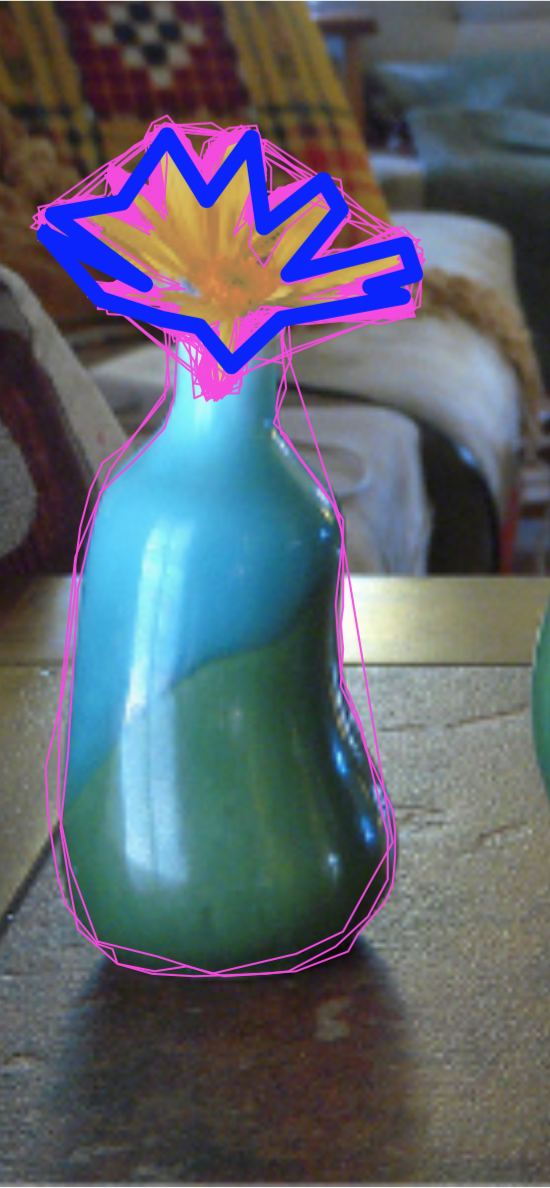
\includegraphics[width=.25\textwidth]{plots/worker_cropped.png}
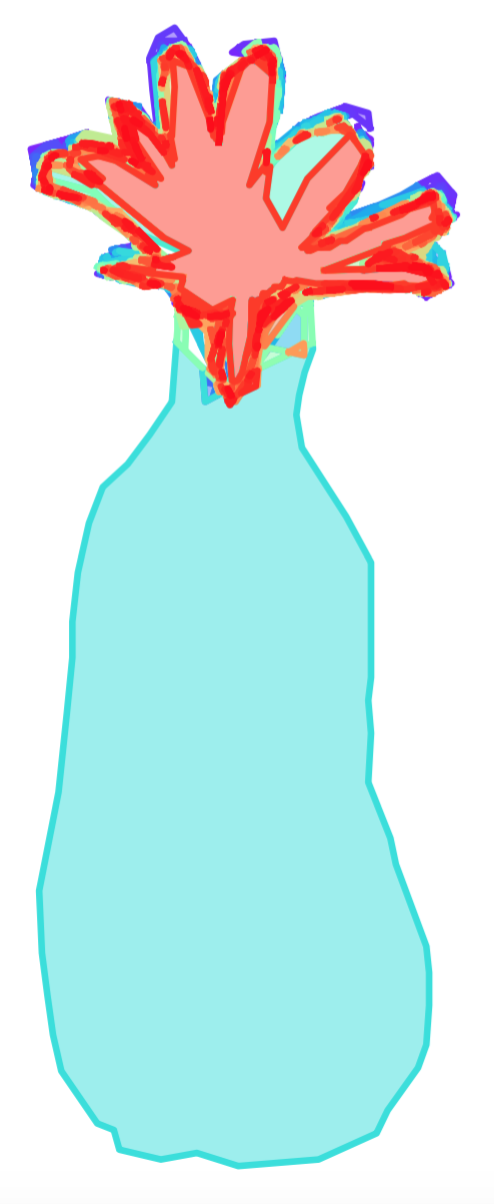
\includegraphics[width=.2\textwidth]{plots/tile_cropped.png}
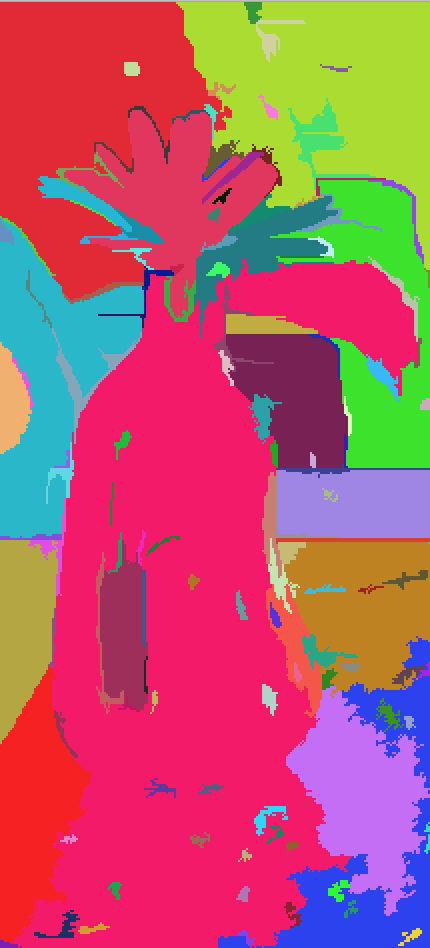
\includegraphics[width=.25\textwidth]{plots/vision_cropped.png}
\caption{Left: Pink shows 40 worker bounding boxes for the object ``flower`` and blue ground truth segmentation, superimposed on the original COCO image. Center: Non-overlapping tiles constructed from worker bounding box. Right: Output from the color-segmentation vision algorithm.}
\label{flower_example}
\todo[inline]{Add black and white, vision segmented region image}
\end{figure}
%Clarify that our search space is tile combination formed by all the worker's tiles not the space of all possible coordinates. (i.e. we assume that a region can not be inside the BB if no workers bounded that region) 
Tiles are finer grained than bounding boxes. Our tile-based approach is inspired by the S-T graph in the classical graph cut problem, where the goal of image segmentation is to find a vertex partition between the object and background regions.\todo[inline]{we don't actually use tile graph here, move to vision section? }

\par $\mathcal{T}=\{t_k\}$ is the set of all non-overlapping tiles for an object i. T is the ground truth tile set. $T^\prime$ is some combination of tiles chosen from $\mathcal{T}$.
 The indicator label $l_{kj}$ is one when worker j votes on the tile $t_{k}$ (i.e. the bounding box that he draws contains $t_{k}$), and zero otherwise. The indicator matrix consisting of tile indicator for all workers is denoted as $\mathbf{l_{kj}}$.

\subsection{Worker Error Model}
We propose three different worker error models describing the probability of a worker j's vote on a specific tile $t_k$, given the tile's inclusion in ground truth and a set of worker qualities $Q_j$. 
\begin{enumerate}
\item Basic: single-parameter Bernoulli model, where $q_j$ is the probability of the worker getting a tile correct. A worker is correct when his vote ($l_{jk}$) matches with the ground truth inclusion of the tile ($t_k\in T$). A worker makes an incorrect response when their vote contradicts with the inclusion of the tile in T ($\{t_k\in$ T$\quad\&\quad l_{kj}=0\}, \{t_k\notin $T$\quad\&\quad l_{kj}=1\}$)
\begin{equation}
p(l_{jk}|t_k\in T, Qj) = \begin{cases}
               q_j, \quad l_{jk}=1\\
               1-q_j, \quad l_{jk}=0\\
            \end{cases}
\end{equation}
\item Large Small Area (LSA): The basic model equally weighs all tiles, but intuitively a worker should be rewarded more if they get a large-area tile correct. We use a two-parameter Bernoulli to model two different tile sizes determined by a threshold $A^*$.
\begin{equation}
p(l_{jk}|t_k\in T,Q_j) = \begin{cases}
               q_{j1}, \quad l_{jk}=1 \& A(t_k)\geq A^*\\
               1-q_{j1}, \quad l_{jk}=0 \& A(t_k)\geq A^*\\
                q_{j2}, \quad l_{jk}=1 \& A(t_k)< A^*\\
               1-q_{j2}, \quad l_{jk}=0 \& A(t_k)< A^*\\
            \end{cases}
\end{equation}
\item Ground truth inclusion, large small area (GTLSA): We observe in our experiment that there can be many large area tiles that lies outside of the ground truth drawn by workers who tend to draw loose, overbounding boxes. Our 4 parameter Bernoulli model distinguishes between false and true positive rates, by taking into account the positive and negative regions (i.e. regions that lies inside or outside of T). 
In the case where $A(t_k)\geq A^*$: 
\begin{equation}
p(l_{jk}|t_k\in T,Q_j) = \begin{cases}
               q_{p1}, \quad l_{jk}=1  \\
               1-q_{p1}, \quad l_{jk}=0  \\
            \end{cases}
\end{equation}
\begin{equation}
p(l_{jk}|t_k\notin T,Q_j) = \begin{cases}
               q_{n1}, \quad l_{jk}=0  \\
               1-q_{n1}, \quad l_{jk}=1  \\
            \end{cases}
\end{equation}
%\item Area-weighted scoring: 
From the worker error model, we can also derive the probability that a tile is in ground truth $p(t_k\in T|Q_j, l_{jk})$ using Bayes rule, assuming the prior probabilities as constant.
\end{enumerate}

\subsection{Problem Statement}
%Describe assumptions on pdfs and inference process. (E and M steps). How are parameters in the models determined empirically.
\par For our problem, we consider only finding tile regions that could be constructed from worker bounding boxes. In other words, our objective is to find the tile combination $T^\prime$ that maximizes the probability that it is the ground truth p($T^\prime$=T), given a set of worker qualities $Q_j$ and tile indicator labels $l_{jk}$: 

\begin{equation}
T = \argmax_{T^\prime \subseteq \mathcal{T}}p(T=T^\prime |  \mathbf{l_{kj}},Q_j)
\label{objective}
\end{equation}
Using Bayes rule we can rewrite this in terms of the posterior probability of the tile-based values($\mathbf{l_{kj}}$) or worker-based values($Q_{j}$), which we can use for the E and M step equations respectively. 
\subsection{Inference}
\par For the E step, we assume T' is ground truth and estimate the $Q_j$ parameters. We can rewrite Eq.\ref{objective} as: 
\begin{equation}
p(T^\prime| Q_j,\mathbf{l_{kj}})
\approx p(l_{kj}| Q,T^\prime)
\end{equation}
where we treat the priors $p(T^\prime),p(Q_j)$ as constants.
Our goal is to find the maximum likelihood parameters of $Q_j$: 
\begin{equation}
\hat{Qj} = \argmax_{Q_j} p(Q_j| \mathbf{l_{kj}},T^\prime)
\end{equation}
% assume p(T') uniform or constant p(Qj), no prior information 
We use the binary random variable w to indicate whether the worker makes a correct vote (w=1) or an incorrect vote(w=0) for a tile. We can write the worker quality probability as the product of the probabilities that they would assume these two independent states (correct/incorrect). 
\begin{align}
p(Q_j) = \prod_j q_j^{p_j(w=1)}\cdot [1-q_j]^{p(w=0)}
\end{align}
The closed form of the maximum likelihood solution for the Bernoulli distribution reduces down to: 
\begin{equation}
\hat{q_j}=\frac{n_{correct}}{n_{total}}
\end{equation}
\par For the M step, we maximize the likelihood of the tile combination $T^\prime$ for a fixed set of worker qualities, $\{Q_j\}$. Following Eq.\ref{objective} from Bayes rule, 
\begin{equation}
p(T^\prime| Q_j,\mathbf{l_{kj}})
\approx p(\mathbf{l_{kj}}|Q_j,l_k)
\end{equation}
% rephrase what your optimization function is, i.e. argmax RHS of equation p(lkj)
Our optimization function is written as:
\begin{equation}
\hat{T^\prime}=\argmax_{T^\prime\supseteq \{T^\prime\} } \prod_j p(\mathbf{l_{kj}}|Q_j,l_k)
\end{equation}
 The product over $T^\prime$ can be further decomposed into its tile components. The likelihoods of these tiles can be computed via the worker error model: 
\begin{equation}
=\argmax_{T^\prime\supseteq \{T^\prime\}} \prod_j\Bigg[\prod_{t_k\in T^\prime} p(t_k\in \mathrm{T}|Q_j,l_k)\prod_{t_k\notin T^\prime} p(t_k\notin \mathrm{T}|Q_j,l_k)\Bigg]
\end{equation}
% * <akashds.iitk@gmail.com> 2017-04-25T02:53:10.683Z:
% 
% The term summing over, $T' \subsetof \mathbf{T} $ can have slightly better notation. Introduce some bold T as space of all possible tile combinations, and use T' subsetof T.
% 
% ^.
\subsubsection{NP-hardness proof}
\subsection{Optimization}
%Explain heuristics used for avoiding to search through all T'. 
Since the space of possible $\{T^{\prime}\}$ to search through is $2^{N}$ where number of tiles (N) for an average object with 30$\sim$40 worker is on the order of thousands, we develop several strategies to narrow the search space for making the problem computationally feasible. 
\subsubsection{High-confidence snowball}
The goal of the snowball method is to come up with smaller subsample of tile combinations $T^\prime$ that are good candidates of ground truth. First, we use tile properties such as area or votes as a heuristic to derive a fixed set of high-confidence tiles as the core. Then, using the same heuristic, we randomly generate subsets from other medium confidence tiles and combined with these core tiles. Tiles picked with such heuristics often have high recall, which means that our TileEM algorithm essentially helps us find a more precise $T^{\prime}$ from $\{T^{\prime}\}$. In our experiment, we define our confidence score as 2$\cdot$votes+area, with 3 high-confidence, fixed core tiles and 40 flexible medium confidence tiles. 
\todo[inline]{NOTE: Might want to consider adjacency-based snowball approach too}
\subsubsection{Maximum likelihood Construction}
Apart from constructing a set of  $\{T^{\prime}\}$ for picking the best  $T^{\prime}$, we can instead directly construct the maximum likelihood tile $T^*$ by choosing tiles that satisfy the criterion: 
\begin{equation}
T^* = \{t_k|p(t_k\in T|l_k,Q_j)\geq p(t_k\notin T|l_k,Q_j)\}
\end{equation}
\subsubsection{Proof:}
We show that this tile-picking heuristic is at least as likely as any tile combination that we would pick with the $\{T^{\prime}\}$ selection method. Suppose there is a $T^\prime$ such that it consists of the same tiles as $T^*$, but we randomly drop a tile $t_{k^\prime}$
\begin{equation}
p(T^*=T^\prime|l_k,Q_j)=\prod_{t_k} p(t_k\in T^*)\cdot p(t_{k^\prime}\notin T^*)
\end{equation}
By definition all tiles in $T^*$ must satisfy $p(t_k\in T|l_k,Q_j)\geq p(t_k\notin T|l_k,Q_j)$, so the dropped tile must have lower probability than $T^\prime$.
\begin{align}
p(T=T^\prime)=p(T^*\setminus t_k^\prime) p(t_k^\prime \notin T^*) \\
% * <akashds.iitk@gmail.com> 2017-04-25T03:02:53.207Z:
% 
% > T^*
% T'
% 
% ^.
p(T=T^*)=p(T^*\setminus t_k^\prime) p(t_k^\prime \in T^*) 
\end{align}
By dropping multiple $t_{k^\prime}$ from $T^*$ or adding $t_{k^\prime}$ not previously in $T^*$, the above result can be generalized to arbitrary $T^\prime$.
\begin{algorithm}[ht!]
 \KwData{fixed $Q_j$}
 %\KwResult{}
 Initialize $T^*$\;
 \For{$t_k \in \mathcal{T}$ }{
  \If{$p(t_k\in T)\geq p(t_k\notin T)$ }{
   $T^*\leftarrow T^* \cup t_k$;
   }
 }
 \caption{M step algorithm. For the initialization of $T^*$, we could start from either an empty set or a high-confidence tileset. The set of $\mathcal{T}$ to chose from can either be the set of all tiles or all tiles adjacent to $T^*$. }\label{Mstep}
\end{algorithm}

\subsection{Our Algorithm}
\todo[inline]{name / abbreviation for algo}
In practice, we desire contiguous bounding boxes. Therefore, we impose an adjacency constraint while choosing our set of optimal tiles. Furthermore, we find that we can trade-off precision for recall by relaxing our condition for choice of tile \todo[inline]{p(tk) $>=$ thresh}.
\begin{algorithm}[ht!]
 \KwData{fixed $Q_j$}
 %\KwResult{}
 $T^*$ = high confidence tiles\;
 $d^\prime$=0\;
 good tile count at $d^\prime$=1\;
 \While{good tile count at $d^\prime \neq 0$}{
 	$\{t_{k,d=d^\prime}\}\leftarrow$ find all tiles at d=$d^\prime$ shell\;
    \For{$t_k \in \{t_{k,d=d^\prime}\}$}{
    	\If{$p(t_k\in T)\geq p(t_k\notin T)$ }{
   			$T^*\leftarrow T^* \cup t_k$\;
            good tile count at $d^\prime$ ++\;
   		}    
 	}
    $d^\prime$++\;
 }
 \caption{Shell-based M step algorithm enforces tiles that are added into $T^*$ must be adjacent to one another.}\label{Mstep}
\end{algorithm}
\subsubsection{Incorporating vision information}
We also use our color-separated segments provided by the vision baseline to improve the output of our algorithm further in a post-processing step.
\todo[inline]{describe}

\section{Experiments}
\subsection{Dataset}
We collected data from Amazon Mechanical Turk where each HIT consisted of one annotation task for a specific pre-labeled object in the image. There is a total of 44 objects in 9 images from the MSCOCO dataset~\cite{Lin2014}. These tasks represent a variety of image difficulty (clutterness, occlusion, lighting)and levels of task ambiguity. For each object, we collected annotations from a total of 40 independent workers. We eliminated all bounding boxes from workers that were self-intersecting. A sub-sampled dataset was created from the full dataset to determine the efficacy of these algorithms on varying number of worker responses, based on Table.\ref{batch_sample}.
\begin{table}[ht]
\centering
\label{batch_sample}
\caption{Every object was randomly sampled worker with replacement. For small worker samples, we average our results over larger number of batches than for large worker samples (which have lower variance, since the sample size is close to the original data size).}
\begin{tabular}{l|llllll}
\# of workers & 5  & 10 & 15 & 20 & 25 & 30 \\ \hline
\# of batches & 10 & 8  & 6  & 4  & 2  & 1 
\end{tabular}
\end{table}
\par The dataset that we have collected is fairly noisy. Average PR against ground truth is ----- and -----MU/STD----- respectively. And while workers have equal rates of overbounding or underbounding behaviours, workers tend to overbound by a larger amount of area ($\mu=7212$) than underbound ($\mu=1306$).  The distributions of worker's bounding box qualities approximately follows a transformed Gaussian(Johnson SU) distribution that accounts for the right-skewed, long-tail characteristics of the distribution.

\subsection{Evaluation Metrics}
 Evaluation metrics used in our experiment measures how well the final bounding box produced by these algorithms compare against ground truth. The most common evaluation metric used in literature are area-based methods which take into account the intersection, $\mathcal{I}=area(z_i\cup z_j)$, or union, $\mathcal{U}=area(z_i\cap z_j)$, between the user and the ground truth bounding boxes.
\begin{align}
\texttt{Precision} = \frac{\mathcal{I}}{area(z_i)} \\
\texttt{Recall} = \frac{\mathcal{I}}{area(z_j)} \\
\texttt{Jaccard} = \frac{\mathcal{U}}{\mathcal{I}}
\end{align}

\subsection{Baselines}

\todo[inline]{Optional: show example of where this fails from vision GT output}
\subsubsection{Vision}
\todo[inline]{Akash}
\subsubsection{Best Summarization}
\par Summarization-based metrics are computable heuristics that measure the quality of a worker's bounding box given the ground truth. We employ two metric used in ~\cite{Vittayakorn2011}, number of control points and annotation size, which has been shown to perform better than vision-based summarization metrics. The number of control points metric is based on the intuition that a more precise bounding box consisting of a large number of control points usually indicates that the user made an effort to closely follow the object boundary. The annotation size is based on the intuition that larger bounding-box-to-image-area ratio means that the object is easier to annotate, hence its quality should be higher.
Both of these metrics optimizes for recall at the cost of precision loss.
\par Summarization based metrics does poorly in cases where the 1-D projection of the BBs fails to capture the worker errors fully. They are good indicators assuming the worker error is only based on the degree of sloppiness of his bounding box rather than mistakes on which regions should be incorporated in the object. For the same reasons, these metric also fail in the case of over-bounding or under-bounding BBs. In practice, quality evaluation is done by setting ground truth to be the bounding box with the best summarization score. The upper limit corresponds to the individual worker with the best summarization score when compared against ground truth.
\subsubsection{Majority Vote variant}
A common strategy for aggregating worker bounding boxes is to pick the majority-voted tile. We investigated three types of variants for majority vote strategies: picking the top-k, top-percentile tiles of vote counts and picking the tiles that were voted by at least 50\% of the workers. We found that among these majority vote variants, the latter strategy gave the highest accuracy.
\todo[inline]{show upper limit to tile-based method $>$ upper limit for summarization based method when Nworker low.}
The upper limit to the 

\subsection{Results}
\todo[inline]{Note: Our TileEM can do better since our tile is slightly overlapping so the tile resolution was not that great.}
\todo[inline]{Re-organize to first compare our algo (with ``best'' param tuning against worker, vision, and gt baselines. Then a separate subsection to explore the variation of our algo with different settings for input parameters.}
\todo[inline]{What's the best way to display P and R separately?}
\begin{table}[ht!]
\begin{tabular}{lrrrr}
\hline
 Number of Workers   &    5 &   10 &   15 &   20 \\
\hline
 P [Num Points]      & 0.88 & 0.79 & 0.77 & 0.80 \\
 R [Num Points]      & 0.89 & 0.81 & 0.81 & 0.84 \\
 P [Area Ratio]      & 0.81 & 0.68 & 0.63 & 0.64 \\
 R [Area Ratio]      & 0.89 & 0.84 & 0.83 & 0.84 \\
 P [GT Precision (*)]    & 0.96 & 0.89 & 0.89 & 0.93 \\
 R [GT Precision (*)]    & 0.87 & 0.78 & 0.76 & 0.77 \\
 P [GT Recall (*)]       & 0.90 & 0.78 & 0.76 & 0.77 \\
 R [GT Recall (*)]       & 0.97 & 0.90 & 0.89 & 0.93 \\
 P [GT Jaccard]      & 0.95 & 0.87 & 0.87 & 0.90 \\
 R [GT Jaccard]      & 0.96 & 0.87 & 0.87 & 0.91 \\
 \hline
 P [Vision GT 50\%]   & 0.92 & 0.90 & 0.90 & 0.90 \\
 R [Vision GT 50\%]   & 0.86 & 0.74 & 0.74 & 0.75 \\
 \hline
 P [TileEM thres=40] & 0.93 & 0.93 & 0.94 & 0.95 \\
 R [TileEM thres=40] & 0.97 & 0.93 & 0.93 & 0.88 \\
 P [MVT]             & 0.85 & 0.82 & 0.80 & 0.79 \\
 R [MVT]             & 0.81 & 0.57 & 0.48 & 0.38 \\
 P [GT Tile-Based]  & ? & ? & ? &? \\
 R [GT Tile-Based]  & ? & ? & ? &? \\
\hline
\end{tabular}
\caption{Average precision recall compared against ground truth over all objects between Tile EM and vision, individual worker baselines. For the first 5 summarization based method, we pick the best bounding box based on that metric. Only the Num Point, Area Ratio and Vision algorithm doesn't require ground truth to compute.}
\end{table}
\begin{figure}
\centering
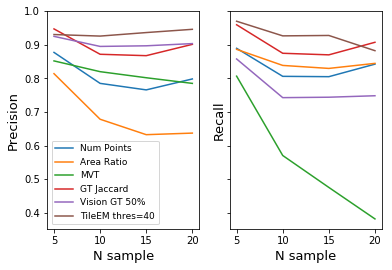
\includegraphics[width=\linewidth]{plots/PRSample2.png}
\caption{Precision recall as number of workers vary.}
\label{PRsample}
\end{figure}
\begin{figure}
\centering
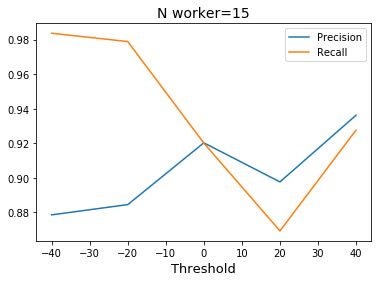
\includegraphics[width=\linewidth]{plots/TileEMThreshold.png}
\caption{Tile EM Precision Recall as the threshold for inclusion criterion in ML construction varies.}
\label{TileEMThreshold}
\end{figure}
% \begin{table*}[ht]
% \begin{tabular}{lrrrrrr}
% \hline
%            &   Num Points &   Area Ratio &   Jaccard [Self] &   Precision [Self] &   Recall [Self] &   Vision \\
% \hline
%  Precision &         0.71 &         0.56 &             0.95 &               0.98 &            0.73 &     0.91 \\
%  Recall    &         0.84 &         0.87 &             0.95 &               0.76 &            0.99 &     0.74 \\
% \hline
% \end{tabular}
% \todo[inline]{NOTE: Will add additional columns from our TileEM algorithm later.}
% \end{table*}

\begin{itemize}
\item plot PR curves for each algorithm, compute AUC
\item PR values in a table of all algorithms compared against baseline
\item show that our experiment works well on smaller, noisier datasets
\item Baselines: 
\begin{itemize}
\item summarization-based methods
\begin{itemize}
\item Jaccard, PR
\item Heuristics: NumPts, Area
\end{itemize}
\item tile based majority vote 
\item color-based computer vision
\item Individual worker responses
\end{itemize}
\end{itemize}
\section{Conclusion}
- Future work: model task difficulty and worker qualities across tasks

\bibliographystyle{named}
\bibliography{reference}
\end{document}